\documentclass[a4paper,11pt]{article}
\usepackage{geometry}
\usepackage{amsmath}
\usepackage{amssymb}
\usepackage{array}
\usepackage{tabularx}
\usepackage{setspace}
\usepackage{graphicx} % Required for including images
\usepackage{tikz}     % Required for watermarking and shapes
\usepackage{fancyhdr} % Required for custom headers/footers
\usepackage{xcolor}
\usepackage{tcolorbox}

\geometry{a4paper, margin=1in}
\setlength{\headheight}{33pt} % Fix header height for logo
\addtolength{\topmargin}{-21pt} % Adjust top margin accordingly

% --- Watermark setup ---
\usepackage{eso-pic}
\newcommand\BackgroundPicture{%
\put(\LenToUnit{0.5\paperwidth},\LenToUnit{0.5\paperheight}){%
\makebox(0,0)[c]{%
\tikz[opacity=0.08]\node{\includegraphics[width=1\paperwidth]{../oatutors_logo.png}};%
}%
}}
\AddToShipoutPicture{\BackgroundPicture}
% --- End Watermark setup ---

% --- Header setup for logo ---
\pagestyle{fancy}
\fancyhf{} % Clear all header and footer fields
\fancyhead[L]{\includegraphics[height=1.0cm]{../oatutors_logo.png}} % Logo on the left (slightly smaller for better proportion)
\fancyhead[C]{\textbf{11+ Non-Verbal Reasoning - Student Notes}} % Course title in center
\fancyhead[R]{\rightmark} % Section title on the right
\fancyfoot[C]{\thepage} % Page number in the footer
\renewcommand{\headrulewidth}{0.4pt} % Line under the header
\renewcommand{\footrulewidth}{0.4pt} % Line over the footer
% --- End Header setup ---

\begin{document}
\onehalfspacing

% This resets the page counter to 0 for the first page after the header setup
% \thispagestyle{fancy} % Apply fancy style to the first page too

\begin{center}
\textbf{\Large 11+ NVR Student Notes: Shape Puzzles}
\vspace{0.2cm}
\end{center}

\hrule
\vspace{0.1cm}

\textbf{Website:} \texttt{https://oatutors.co.uk/}

\vspace{0.2cm}
\hrule
\vspace{0.3cm}

\begin{tcolorbox}[colback=blue!5!white,colframe=blue!75!black,title=\textbf{What You'll Learn Today}]
\begin{itemize}
    \item Learn how to add shapes together (Collecting Rule)
    \item Master the disappearing trick (Cancellation Rule)
    \item Solve shape puzzles step by step
    \item Recognize patterns in Non-Verbal Reasoning
\end{itemize}
\end{tcolorbox}

\section{Shape Math Magic!}

\begin{tcolorbox}[colback=green!5!white,colframe=green!75!black,title=\textbf{The Big Idea}]
Shapes work like numbers! We can add them together and take them away.
\\
\textbf{Shape 1 + Shape 2 = Shape 3}
\\
\textbf{Shape 1 - Shape 2 = Shape 3}
\end{tcolorbox}

Think of shapes like your toys - you can put them all in one box (adding) or remove the ones that are the same (taking away)!

\section{The Two Super Rules}

\subsection{Rule 1: The Collecting Rule (+)}

\begin{tcolorbox}[colback=orange!5!white,colframe=orange!75!black,title=\textbf{Collecting Rule}]
When we see a \textbf{+} sign, we collect ALL shapes from both boxes and put them in the third box.
\\
It's like putting all your toys in one big toy box!
\end{tcolorbox}

\textbf{Example:} Box with square + Box with circle = Box with BOTH square AND circle

\subsection{Rule 2: The Disappearing Rule ($\leftrightarrow$ or $-$)}

\begin{tcolorbox}[colback=red!5!white,colframe=red!75!black,title=\textbf{Disappearing Rule (Magic Trick!)}]
When we see $\leftrightarrow$ or $-$, shapes that appear in BOTH boxes disappear!
\\
Only shapes that are in just ONE box will stay.
\end{tcolorbox}

\textbf{The Magic:} Same shapes in both boxes = POOF! They vanish! ✨

\section{Step-by-Step Strategy}

\begin{tcolorbox}[colback=purple!5!white,colframe=purple!75!black,title=\textbf{How to Solve Any Shape Puzzle}]
\textbf{Step 1:} Look at the operation sign (+ or $\leftrightarrow$)

\textbf{Step 2:} If it's +, collect all shapes together

\textbf{Step 3:} If it's $\leftrightarrow$, find shapes that appear in BOTH boxes

\textbf{Step 4:} Make the matching shapes disappear

\textbf{Step 5:} Keep only the unique shapes (ones that appear in just ONE box)
\end{tcolorbox}

\section{Visual Examples}

\subsection{Collecting Example}
\begin{center}
\begin{tikzpicture}[scale=0.6]
    % Box 1 with square
    \draw[thick] (0,0) rectangle (1.5,1.5);
    \draw[thick] (0.4,0.4) rectangle (1.1,1.1);
    \node at (0.75,-0.3) {Box 1};
    
    % Plus
    \node at (2,0.75) {\Large +};
    
    % Box 2 with circle
    \draw[thick] (2.5,0) rectangle (4,1.5);
    \fill[black] (3.25,0.75) circle (0.3);
    \node at (3.25,-0.3) {Box 2};
    
    % Equals
    \node at (4.5,0.75) {\Large =};
    
    % Box 3 with both
    \draw[thick] (5,0) rectangle (6.5,1.5);
    \draw[thick] (5.2,0.4) rectangle (5.7,0.9);
    \fill[black] (6.1,1) circle (0.2);
    \node at (5.75,-0.3) {Box 3};
\end{tikzpicture}
\end{center}

\subsection{Disappearing Example}
\begin{center}
\begin{tikzpicture}[scale=0.6]
    % Box 1 with circle and triangle
    \draw[thick] (0,0) rectangle (1.5,1.5);
    \fill[black] (0.5,0.75) circle (0.2);
    \fill[black] (1,1.2) -- (0.8,0.8) -- (1.2,0.8) -- cycle;
    \node at (0.75,-0.3) {Box 1};
    
    % Disappearing symbol
    \node at (2,0.75) {\Large $\leftrightarrow$};
    
    % Box 2 with circle and square
    \draw[thick] (2.5,0) rectangle (4,1.5);
    \fill[black] (3,0.75) circle (0.2);
    \draw[thick] (3.3,0.4) rectangle (3.8,0.9);
    \node at (3.25,-0.3) {Box 2};
    
    % Equals
    \node at (4.5,0.75) {\Large =};
    
    % Box 3 with only triangle and square (circle disappeared!)
    \draw[thick] (5,0) rectangle (6.5,1.5);
    \fill[black] (5.4,1.2) -- (5.2,0.8) -- (5.6,0.8) -- cycle;
    \draw[thick] (5.9,0.4) rectangle (6.2,0.7);
    \node at (5.75,-0.3) {Box 3};
\end{tikzpicture}
\end{center}

\textbf{Why?} The circle appeared in BOTH Box 1 and Box 2, so it disappeared! Only the triangle (from Box 1) and square (from Box 2) remained.

\section{Quick Practice Tips}

\begin{itemize}
    \item \textbf{For Collecting (+):} Count all shapes and put them together
    \item \textbf{For Disappearing ($\leftrightarrow$):} Put your finger on matching shapes - they vanish!
    \item \textbf{Look carefully:} Same shape, same color, same size = they match
    \item \textbf{Different shapes:} Circle ≠ Square ≠ Triangle ≠ Star
    \item \textbf{Different colors:} Black ≠ White ≠ Gray
\end{itemize}

\section{Common Mistakes to Avoid}

\begin{tcolorbox}[colback=yellow!10!white,colframe=orange!50!black,title=\textbf{Watch Out!}]
\begin{itemize}
    \item ❌ Forgetting to check the operation sign
    \item ❌ Not noticing small differences in shapes
    \item ❌ Mixing up collecting and disappearing rules
    \item ❌ Not checking colors carefully (black vs white vs gray)
    \item ❌ Rushing - take time to compare each shape
\end{itemize}
\end{tcolorbox}

\section{Memory Tricks}

\begin{itemize}
    \item \textbf{Collecting Rule:} Think "collection box" - everything goes in!
    \item \textbf{Disappearing Rule:} Think "magic trick" - identical twins vanish!
    \item \textbf{Operation Signs:} + = collect, $\leftrightarrow$ = cancel out
    \item \textbf{Matching:} Same shape + same color + same size = MATCH!
\end{itemize}

\section{Quick Practice}

Try to solve these puzzles using our rules:

\textbf{Puzzle 1:} What happens when you collect a star and a circle together?

\textbf{Puzzle 2:} You have two boxes: Box A has a black square and white circle. Box B has a black square and gray triangle. Using the disappearing rule, what's left?

\textbf{Puzzle 3:} Look for this pattern in your next worksheet: Box 1 + Box 2 = ?

\vspace{1cm}

\begin{tcolorbox}[colback=gray!10!white,colframe=gray!50!black,title=\textbf{Success Tips}]
\begin{itemize}
    \item Practice identifying shapes quickly
    \item Always check the operation sign first
    \item Use your finger to track matching shapes
    \item Take your time - accuracy beats speed!
    \item Ask for help if you get stuck
\end{itemize}
\end{tcolorbox}

\section{Next Steps}

\begin{itemize}
    \item Master these two rules with lots of practice
    \item Look for more complex patterns with multiple shapes
    \item Practice with different colors and sizes
    \item Challenge yourself with harder puzzles!
\end{itemize}

\end{document}